% Plantilla LaTeX convertida desde:
% Tecnologia_en_Marcha/Plantilla artículos Tecnología en marcha-OTH.docx
%
% Compilación con pdfLaTeX (se requieren dos pasadas para resolver las citas):
%
% Desde Tecnologia_en_Marcha/latex_template/:
%   pdflatex plantilla_tecnologia_en_marcha.tex
%   pdflatex plantilla_tecnologia_en_marcha.tex
%
% Desde la raíz del repositorio (los archivos de salida quedarán junto al .tex):
%   pdflatex -output-directory=Tecnologia_en_Marcha/latex_template Tecnologia_en_Marcha/latex_template/plantilla_tecnologia_en_marcha.tex
%   pdflatex -output-directory=Tecnologia_en_Marcha/latex_template Tecnologia_en_Marcha/latex_template/plantilla_tecnologia_en_marcha.tex
%
% Alternativa con latexmk desde la raíz:
%   latexmk -pdf -cd Tecnologia_en_Marcha/latex_template/plantilla_tecnologia_en_marcha.tex

\documentclass[12pt,letterpaper]{article}

% Idiomas y codificación
\usepackage[utf8]{inputenc}
\usepackage[T1]{fontenc}
\usepackage[main=spanish,english]{babel}

% Carlito es una alternativa libre y compatible con métricas de Calibri.
\usepackage[sfdefault]{carlito}
% La excepción evita una advertencia causada por la redefinición de listas de
% la clase article; el resto de las mejoras microtipográficas permanece activo.
\usepackage[nopatch=item]{microtype}

% Márgenes de la plantilla original: carta, 3 cm laterales, 2.5 cm superior/inferior
\usepackage[
  letterpaper,
  left=3cm,
  right=3cm,
  top=2.5cm,
  bottom=2.5cm,
  footskip=1.25cm
]{geometry}

% Formato general
\usepackage{xcolor}
\usepackage{titlesec}
\usepackage{graphicx}
\usepackage{array}
\usepackage{amsmath}
\usepackage{caption}
\usepackage{placeins}
\usepackage{fancyhdr}
\usepackage{siunitx}
\usepackage{cite}
\usepackage{hyperref}

\definecolor{temblue}{HTML}{2F5496}

\setlength{\parindent}{0pt}
\setlength{\parskip}{0.55\baselineskip}
\setcounter{secnumdepth}{0}
\urlstyle{same}

% Formato de números y unidades: coma decimal y espacio fino para millares.
\sisetup{
  output-decimal-marker={,},
  group-separator={\,},
  group-minimum-digits=4,
  detect-all
}

% Permite compilar desde esta carpeta o desde la raíz del repositorio.
\graphicspath{{./}{Tecnologia_en_Marcha/latex_template/}}

% Encabezados y pies: número de página a la derecha, como en la plantilla Word.
\pagestyle{fancy}
\fancyhf{}
\fancyfoot[R]{\thepage}
\renewcommand{\headrulewidth}{0pt}
\renewcommand{\footrulewidth}{0pt}

% Títulos de sección: equivalentes al estilo "Título 2" del DOCX.
\titleformat{\section}
  {\normalfont\color{temblue}\fontsize{13}{15}\selectfont}
  {}{0pt}{}
\titlespacing*{\section}{0pt}{0.75\baselineskip}{0.25\baselineskip}

\titleformat{\subsection}
  {\normalfont\color{temblue}\fontsize{12}{14}\selectfont}
  {}{0pt}{}
\titlespacing*{\subsection}{0pt}{0.6\baselineskip}{0.2\baselineskip}

% Leyendas: "Figura" y "Cuadro", con etiqueta en negrita y punto separador.
\addto\captionsspanish{%
  \renewcommand{\figurename}{Figura}%
  \renewcommand{\tablename}{Cuadro}%
  \renewcommand{\refname}{Referencias}%
}
\captionsetup{
  labelfont=bf,
  labelsep=period,
  justification=centering,
  singlelinecheck=false
}
\captionsetup[table]{name=Cuadro,position=top}

% Metadatos editables del artículo. Actualícelos antes de generar el PDF final.
\newcommand{\TEMtitleES}{Título en español del artículo}
\newcommand{\TEMtitleEN}{Title of the article in English}
\newcommand{\TEMpdfauthors}{Nombre completo de autor 1; Nombre completo de autor 2; Nombre completo de autor 3}
\newcommand{\TEMpdfkeywords}{palabra clave 1; palabra clave 2; palabra clave 3; palabra clave 4; palabra clave 5}

\hypersetup{
  hidelinks,
  unicode=true,
  pdfencoding=auto,
  psdextra,
  pdftitle={\TEMtitleES},
  pdfsubject={Artículo científico para la revista Tecnología en Marcha},
  pdfauthor={\TEMpdfauthors},
  pdfkeywords={\TEMpdfkeywords}
}

% Comandos auxiliares de la plantilla
\newcommand{\TEMtitle}[1]{%
  \begin{center}
    {\fontsize{28}{32}\selectfont #1\par}
  \end{center}
}

% Argumentos: nombre, afiliación y país, correo, URL completa de ORCID.
% \nolinkurl permite mostrar de forma segura correos con caracteres como "_".
\newcommand{\TEMauthor}[4]{%
  \noindent\textbf{#1}\\
  #2\\
  \href{mailto:#3}{\nolinkurl{#3}}\\
  ORCID: \href{#4}{\nolinkurl{#4}}\par
  \vspace{0.25\baselineskip}
}

\begin{document}

% El título debe ser preciso y acorde con los resultados. Evite frases que no
% describan el artículo. Si deriva de una tesis, no se recomienda reutilizar
% exactamente el título de la tesis.
\TEMtitle{\TEMtitleES}

\TEMtitle{\foreignlanguage{english}{\TEMtitleEN}}

\vspace{0.5\baselineskip}

% Afiliación: indique el lugar de trabajo y el nombre completo de la institución;
% no use siglas. Si no posee ORCID, puede crearlo en https://orcid.org.
% El cuarto argumento debe contener la URL completa: https://orcid.org/0000-....
\TEMauthor{Nombre completo de autor 1}{Nombre completo de la institución. País}{autor_1@institucion.ac.cr}{https://orcid.org/0000-0000-0000-0000}
\TEMauthor{Nombre completo de autor 2}{Nombre completo de la institución. País}{autor_2@institucion.ac.cr}{https://orcid.org/0000-0000-0000-0000}
\TEMauthor{Nombre completo de autor 3}{Nombre completo de la institución. País}{autor_3@institucion.ac.cr}{https://orcid.org/0000-0000-0000-0000}

\section{Resumen}
% Se recomienda elaborar el resumen al final de la redacción. Esta sección es
% decisiva para que el lector continúe la lectura del artículo.
El resumen debe estar compuesto por un máximo de 250 palabras y un mínimo de 150 palabras. Debe ser claro y exponer lo más relevante del artículo en cuanto a problema, metodología, resultados y conclusiones.

\section{Palabras clave}
Incluir de 5 a 7 palabras clave separadas por punto y coma (;). No deben ser un recorte del título; deben describir los elementos más importantes del artículo. Usar términos de un tesauro especializado del área, como el de la UNESCO: \url{http://vocabularies.unesco.org/browser/thesaurus/es/}

% Sustituya la instrucción siguiente por la traducción en inglés. Mantenga el
% contenido final dentro de otherlanguage para aplicar las reglas lingüísticas.
\begin{otherlanguage}{english}
\section{Abstract}
\foreignlanguage{spanish}{Traducción fiel del resumen en español. Evitar el uso de traductores automáticos.}

\section{Keywords}
\foreignlanguage{spanish}{Traducción fiel de las palabras clave en español. Evitar el uso de traductores automáticos.}
\end{otherlanguage}

\section{Introducción}
% Plantee el porqué del artículo y proporcione el contexto necesario para que el
% lector comprenda la problemática abordada.
En esta sección del artículo se deben introducir los conceptos necesarios para identificar el problema o situación a resolver. Además, se debe especificar el objetivo de la investigación.

Todas las ideas y conceptos deben estar fundamentados con su correspondiente cita bibliográfica.

% Tecnología en Marcha aplica revisión antiplagio. Cite correctamente todas las
% fuentes, use comillas cuando corresponda y autocite trabajos previos propios
% para evitar plagio intencional o accidental, paráfrasis inadecuada y autoplagio.
De ser necesario, puede incluir otras secciones o subsecciones antes de la metodología.

\section{Materiales y métodos (metodología)}
En esta sección se debe describir de forma detallada la metodología de la investigación. Incluya tipo de investigación, lugar, población, tamaño de muestra, etc.

\section{Resultados}
Se deben describir los resultados obtenidos con la aplicación de la metodología descrita en la sección anterior. Debe apoyarse con cuadros y gráficos, los cuales deben estar debidamente citados en el texto y con numeración consecutiva. Recuerde justificar cada cuadro, ecuación y gráfico incluido, y evitar información redundante.

Como ejemplo de citación interna, la figura \ref{fig:ejemplo} presenta un resultado gráfico, la ecuación \eqref{eq:ejemplo} formaliza la relación analizada y el cuadro \ref{tab:ejemplo} resume los datos correspondientes. Sustituya este texto por la explicación y justificación de cada elemento en su artículo.

% Las figuras deben incluirse en el documento y enviarse además por separado en
% formato .jpg, .ai o .png. Si la figura es de elaboración propia, omita la fuente.
\begin{figure}[htbp]
  \centering
  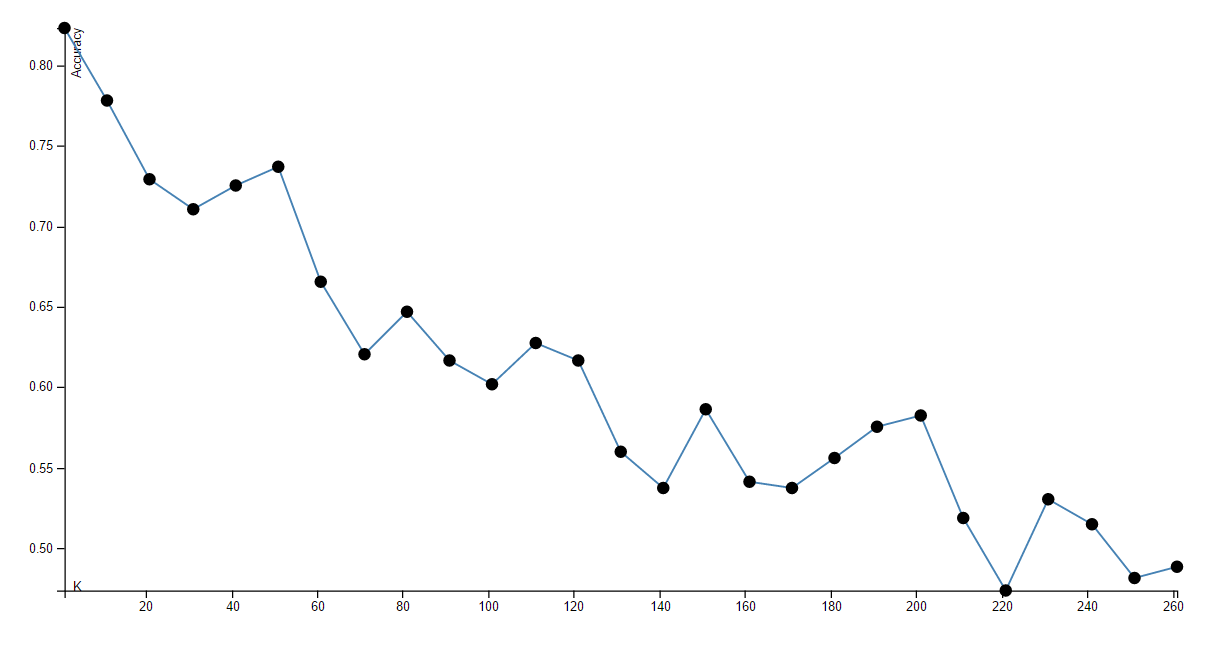
\includegraphics[width=0.75\textwidth]{figura_ejemplo.png}
  \caption{Descripción clara y concisa de la figura 1. Fuente: \cite{oviedo2024}.}
  \label{fig:ejemplo}
\end{figure}

\begin{equation}
  \frac{B}{R_a}=\theta_0 J_0\sqrt[b]{\delta_0}
  \label{eq:ejemplo}
\end{equation}

% Si el cuadro es de elaboración propia, omita la línea "Fuente".
\begin{table}[htbp]
  \centering
  \caption{Descripción clara y concisa del cuadro 1.}
  \label{tab:ejemplo}
  \resizebox{\textwidth}{!}{%
  \begin{tabular}{|l|*{4}{S[table-format=4.2]}|*{4}{S[table-format=4.2]}|}
    \hline
    & \multicolumn{4}{c|}{Marzo 2023} & \multicolumn{4}{c|}{Marzo 2024} \\
    \hline
    Parámetro
      & \multicolumn{1}{c}{Promedio}
      & \multicolumn{1}{c}{Máximo}
      & \multicolumn{1}{c}{Mínimo}
      & \multicolumn{1}{c|}{Desviación estándar}
      & \multicolumn{1}{c}{Promedio}
      & \multicolumn{1}{c}{Máximo}
      & \multicolumn{1}{c}{Mínimo}
      & \multicolumn{1}{c|}{Desviación estándar} \\
    \hline
    DQO (\si{\milli\gram\per\litre})              & 2299.00 & 3438.00 & 1771.00 & 409.99 & 2356.14 & 3094.00 & 1829.00 & 355.07 \\
    DBO$_5$ (\si{\milli\gram\per\litre})        & 1393.84 & 1920.00 & 1017.00 & 232.76 & 1370.48 & 1794.00 &  985.00 & 208.43 \\
    Aceites y grasas (\si{\milli\gram\per\litre}) &  165.69 &  261.00 &   12.00 &  53.40 &  166.93 &  285.00 &   26.00 &  66.70 \\
    SST (\si{\milli\gram\per\litre})            &  712.55 & 1055.00 &  448.00 & 163.18 &  764.81 &  890.00 &  650.00 &  68.84 \\
    Ssed (\si{\milli\litre\per\litre})          &   12.53 &   25.00 &    5.50 &   5.07 &   12.01 &   24.00 &    5.00 &   4.20 \\
    pH                                                &    6.31 &    7.20 &    5.00 &   0.61 &    6.58 &    8.50 &    5.50 &   0.88 \\
    \hline
  \end{tabular}%
  }
  \caption*{\raggedright Fuente: \cite{solorzano2021}.}
\end{table}

% Evita que figuras o cuadros de Resultados aparezcan dentro de otra sección.
\FloatBarrier

\section{Conclusiones y/o recomendaciones (discusión)}
En este apartado se deben indicar las conclusiones y/o recomendaciones derivadas de los resultados obtenidos. También se puede incluir un apartado de discusión donde se confirmen o refuten resultados de acuerdo con la literatura existente. Deben ser claras y evidenciar el aporte del artículo.

\section{Agradecimientos}
Esta sección es opcional y se debe incluir antes de las referencias.

% Las referencias deben aparecer al final, ordenadas según el formato IEEE.
% Incluya únicamente las referencias citadas en el texto. Deben ser actuales
% (no mayores a cinco años) y proceder de fuentes confiables; evite páginas web
% o documentos cuya procedencia no esté claramente identificada.
\begin{thebibliography}{99}

\bibitem{oviedo2024}
A. Oviedo Muñoz, ``Desarrollo de un prototipo para recopilación y monitoreo remoto de datos hídricos de los tanques, basado en dispositivos IoT, en la ASADA Paso Ancho y Boquerón'', trabajo final de graduación, Instituto Tecnológico de Costa Rica, Cartago, Costa Rica, 2024.

\bibitem{solorzano2021}
S. Solórzano Alfaro, ``Sistema de control y monitoreo hídrico, basado en LoRaWAN\textsuperscript{TM}, para el acueducto principal de la Asociación Administradora del Acueducto Rural de Playa Sámara de Nicoya'', trabajo final de graduación, Instituto Tecnológico de Costa Rica, Cartago, Costa Rica, 2021. \url{https://hdl.handle.net/2238/13234}

\end{thebibliography}

\end{document}
